\appendix
\chapter{Một số Model chuẩn}\label{models}

\section{Foundation models}
Foundation models have been defined in the core specification. Two of them are mandatory for all mesh nodes.

\begin{itemize}
	\item Configuration Server (mandatory)
	\item Configuration Client
	\item Health Server (mandatory)
	\item Health Client
\end{itemize}

\section{Generic models}
\begin{itemize}
\item Generic OnOff Server, used to represent devices that do not fit any of the model descriptions defined but support the generic properties of On/Off
\item Generic Level Server, keeping the state of an element in a 16-bit signed integer
\item Generic Default Transition Time Server, used to represent a default transition time for a variety of devices
\item Generic Power OnOff Server \& Generic Power OnOff Setup Server, used to represent devices that do not fit any of the model descriptions but support the generic properties of On/Off
\item Generic Power Level Server \& Generic Power Level Setup Server, including a Generic Power Actual state, a Generic Power Last state, a Generic Power Default state and a Generic Power Range state
\item Generic Battery Server, representing a set of four values representing the state of a battery
\item Generic Location Server \& Generic Location Setup Server, representing location information of an element, either global (Lat/Lon) or local
\item Generic User/Admin/Manufacturer/Client Property Server, representing any value to be stored by an element
\item Generic OnOff Client \& Generic Level Client
\item Generic Default Transition Time Client
\item Generic Power OnOff Client \& Generic Power Level Client
\item Generic Battery Client
\item Generic Location Client
\item Generic Property Client
\end{itemize}

\section{Sensors}
\begin{itemize}
\item Sensor Server \& Sensor Setup Server, representing a sensor device. Sensor device may be configured to return a measured value periodically or on request; measurement period (cadence) may be configured to be fixed or to change, so that more important value range is being reported faster.
\item Sensor Client
\end{itemize}

\section{Time and scenes}
\begin{itemize}
\item Time Server \& Time Setup Server, allowing for time synchronization in mesh network
\item Scene Server \& Scene Setup Server, allowing for up to 65535 scenes to be configured and recalled when needed.
\item Scheduler Server \& Scheduler Setup Server
\item Time Client, Scene Client \& Scheduler Client
\end{itemize}

\section{Lighting}
\begin{itemize}
\item Light Lightness Server \& Light Lightness Setup Server, representing a dimmable light source
\item Light CTL Server, Light CTL Temperature Server \& Light CTL Setup Server, representing a CCT or "tunable white" light source
\item Light HSL Server, Light HSL Hue Server, Light HSL Saturation Server \& Light HSL Setup Server, representing a light source based on Hue, Saturation, Lightness color representation
\item Light xyL Server \& Light xyL Setup Server, representing a light source based on modified CIE xyY color space.
\item Light LC (Lightness Control) Server \& Light LC Setup Server, representing a light control device, able to control Light Lightness model using an occupancy sensor and ambient light sensor. It may be used for light control scenarios like Auto-On, Auto-Off and/or Daylight Harvesting.
\item Light Lightness Client, Light CTL Client, Light HSL Client, Light xyL Client \& Light LC Client
\end{itemize}

\chapter{Flowchart quá trình remote provisioning}\label{remoteprov}
    \begin{figure}[h!]
    	\begin{center}
    		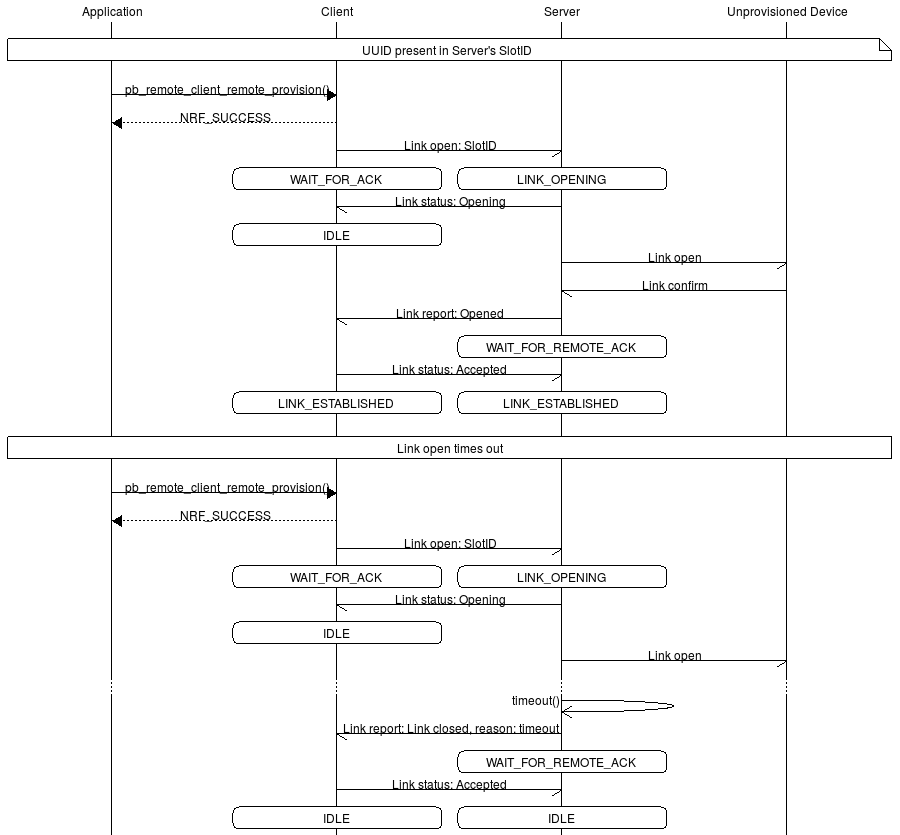
\includegraphics[scale=0.4]{images/msc_pb_remote_link_open.png}
    		\caption{Quá trình remote provisioning}
    	\end{center}
    \end{figure}
    
\chapter{Hướng dẫn thực thi ứng dụng}\label{guide}
\begin{enumerate}
\item Sau khi kết nối Kit PCA10040 với máy tính, sử dụng phần mềm nRFgo Studio để nạp Softdevice cho Kit.
            \begin{figure}[h!]
    	 \begin{center}
    		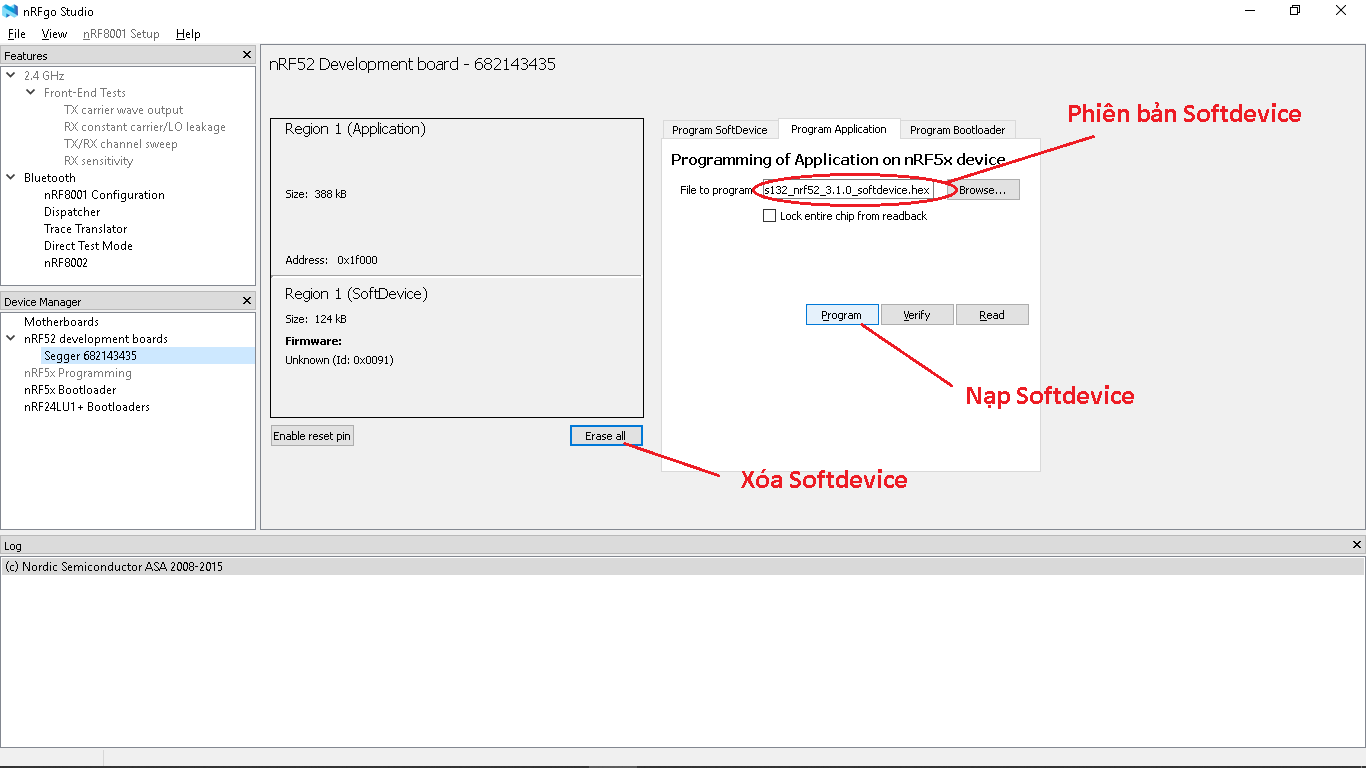
\includegraphics[scale=0.4]{images/app3-1.png}
    		\caption{Giao diện phần mềm nRFgo Studio}
    	\end{center}
    	\end{figure}
\item Sau khi đã nạp Softdevice, tiến hành nạp các chương trình khác nhau cho node cảm biến và node gateway. Node cảm biến sẽ dùng project - Embedded Studio Project - server còn node gateway sẽ dùng project client.
            \begin{figure}[h!]
    	 \begin{center}
    		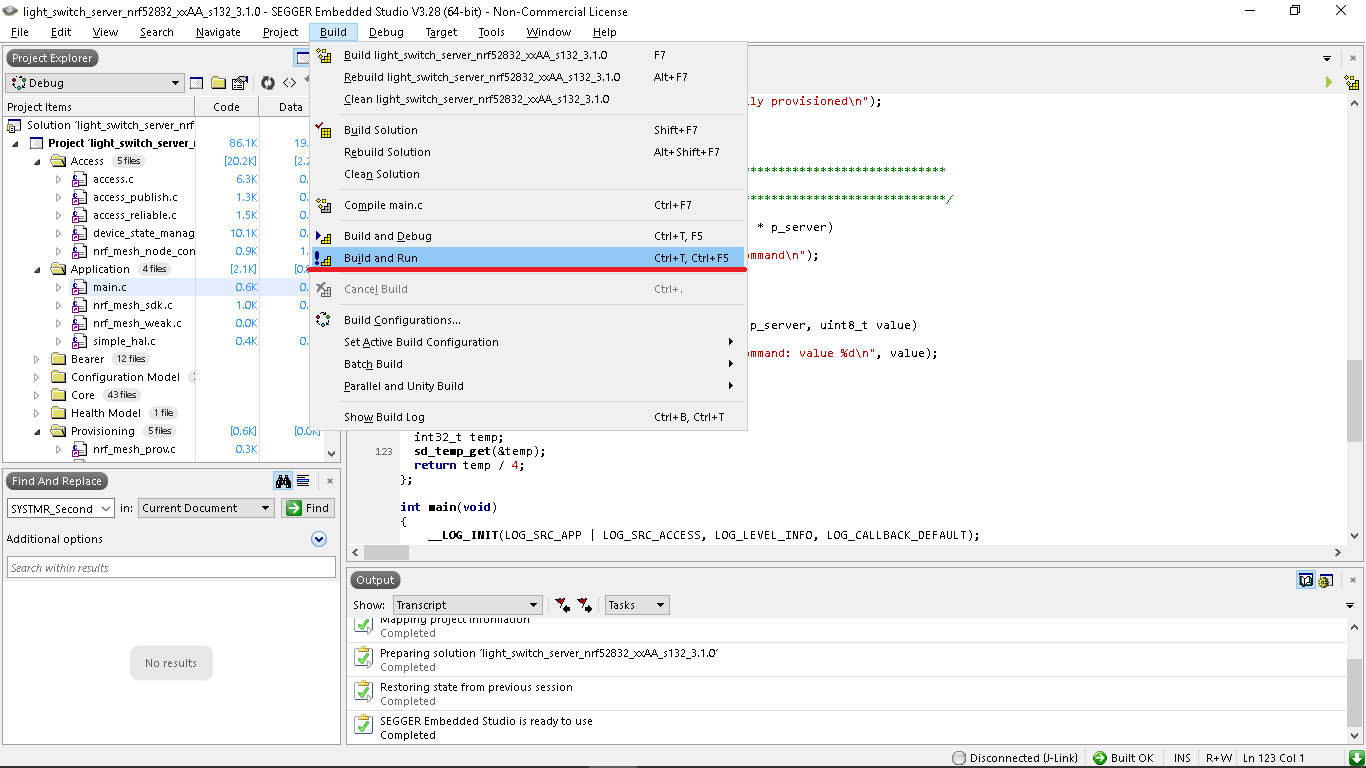
\includegraphics[scale=0.4]{images/app3-2.png}
    		\caption{Giao diện phần mềm Embedded Studio Project}
    	\end{center}
    	\end{figure}
    	\newpage
\item Để theo dõi quá trình thực thi của chương trình, sử dụng J-link RTT Viewer để xem quan sát quá trình.
	 \begin{figure}[h!]
    	 \begin{center}
    		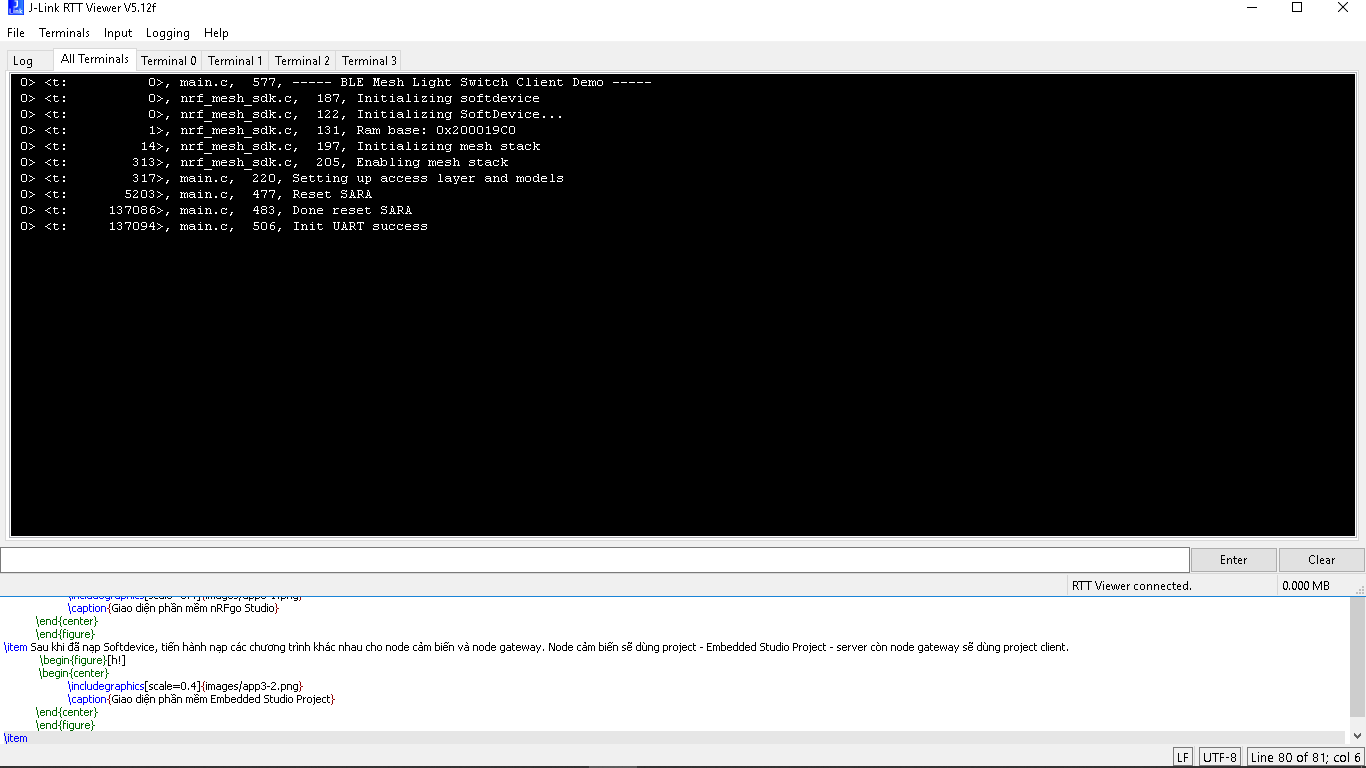
\includegraphics[scale=0.4]{images/app3-3.png}
    		\caption{Giao diện phần mềm J-link RTT Viewer}
    	\end{center}
    	\end{figure}
\end{enumerate}